\documentclass[tikz,border=10pt]{standalone}
\usepackage[T1]{fontenc}
\usepackage{helvet}
\renewcommand{\familydefault}{\sfdefault}
\usepackage{amsmath,amssymb}
\usepackage{tikz}
\usetikzlibrary{calc,positioning,fit,arrows.meta,shapes.geometric}

% Canonical Academic Palette
\definecolor{OxfordNavy}{HTML}{1E293B}
\definecolor{SlateSteel}{HTML}{334155}
\definecolor{MutedTeal}{HTML}{0F766E}
\definecolor{TealL0}{HTML}{F0FDFA}
\definecolor{Burgundy}{HTML}{991B1B}
\definecolor{BurgundyL0}{HTML}{FEF2F2}
\definecolor{WarmOchre}{HTML}{92400E}
\definecolor{OchreL0}{HTML}{FFFBEB}
\definecolor{ForestSage}{HTML}{166534}
\definecolor{SageL0}{HTML}{F0FDF4}
\definecolor{CoolParchment}{HTML}{F8FAFC}
\definecolor{SlateRim}{HTML}{CBD5E1}
\definecolor{GridGray}{HTML}{E2E8F0}
\definecolor{DarkSlate}{HTML}{0F172A}
\definecolor{Amethyst}{HTML}{6B21A8}
\definecolor{AmethystL0}{HTML}{FAF5FF}

\begin{document}
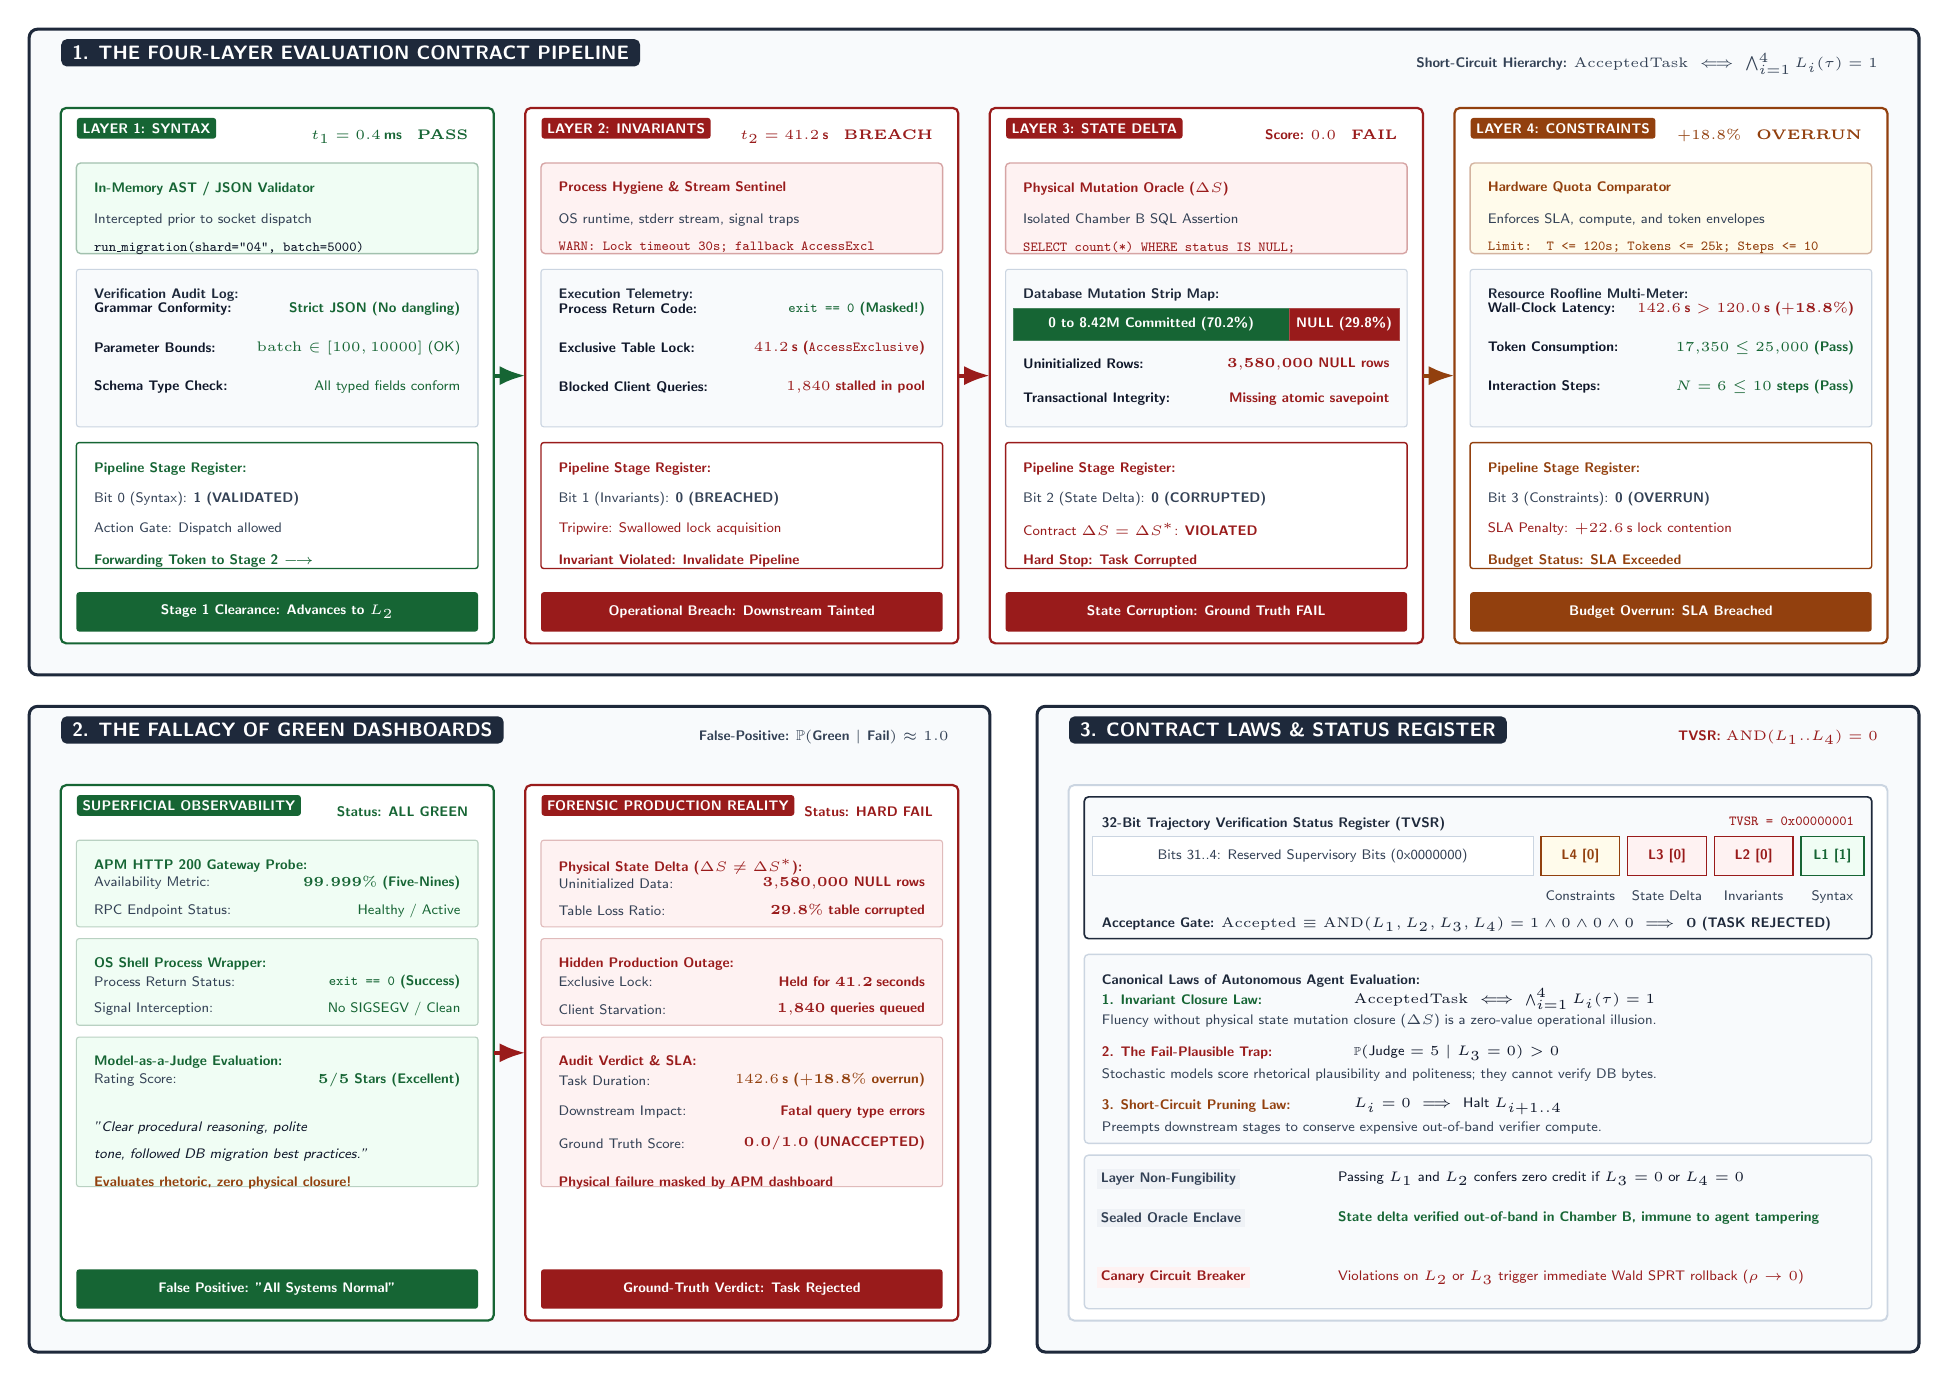
\begin{tikzpicture}[x=1cm, y=1cm, >=Latex]

% =============================================================================
% PANEL 1: THE FOUR-LAYER EVALUATION CONTRACT DATAPATH (TOP)
% (x: 0 to 24.0, y: 8.6 to 16.8) - Height 8.2 cm
% =============================================================================
\begin{scope}[shift={(0, 8.6)}]
  % Base Canvas Container
  \draw[fill=CoolParchment, draw=OxfordNavy, line width=1.1pt, rounded corners=3pt]
    (0, 0) rectangle (24.0, 8.2);

  % 4 Pipeline Stages (x: 0.4, 6.2, 12.0, 17.8; width: 5.6 cm each, gap 0.2 cm)
  % --- STAGE 1: LAYER 1 SYNTAX (x: 0.4 to 5.9) ---
  \begin{scope}[shift={(0.4, 0.4)}]
    \draw[fill=white, draw=ForestSage, line width=0.8pt, rounded corners=2pt] (0, 0) rectangle (5.5, 6.8);

    \node[anchor=north west, fill=ForestSage, text=white, font=\fontsize{5.2}{6.2}\selectfont\bfseries, rounded corners=1pt, inner sep=2pt]
      at (0.2, 6.68) {LAYER 1: SYNTAX};
    \node[anchor=north east, font=\fontsize{4.6}{5.4}\selectfont\bfseries, text=ForestSage]
      at (5.3, 6.65) {$t_1 = 0.4\,\text{ms} \quad \mathbf{PASS}$};

    % Target Box
    \draw[fill=SageL0, draw=ForestSage!40, line width=0.5pt, rounded corners=1.5pt] (0.2, 4.95) rectangle (5.3, 6.10);
    \node[anchor=north west, font=\fontsize{4.8}{5.6}\selectfont\bfseries, text=ForestSage] at (0.3, 5.98) {In-Memory AST / JSON Validator};
    \node[anchor=north west, font=\fontsize{4.2}{5.0}\selectfont, text=SlateSteel] at (0.3, 5.58) {Intercepted prior to socket dispatch};
    \node[anchor=north west, font=\fontsize{4.2}{5.0}\selectfont\ttfamily, text=DarkSlate] at (0.3, 5.22) {run\_migration(shard="04", batch=5000)};

    % Hardware Register
    \draw[fill=CoolParchment, draw=SlateRim, line width=0.4pt, rounded corners=1pt] (0.2, 2.75) rectangle (5.3, 4.75);
    \node[anchor=north west, font=\fontsize{4.5}{5.2}\selectfont\bfseries, text=OxfordNavy] at (0.3, 4.62) {Verification Audit Log:};

    \node[anchor=west, font=\fontsize{4.2}{5.0}\selectfont\bfseries, text=DarkSlate] at (0.3, 4.25) {Grammar Conformity:};
    \node[anchor=east, font=\fontsize{4.2}{5.0}\selectfont\bfseries, text=ForestSage] at (5.2, 4.25) {Strict JSON (No dangling)};

    \node[anchor=west, font=\fontsize{4.2}{5.0}\selectfont\bfseries, text=DarkSlate] at (0.3, 3.75) {Parameter Bounds:};
    \node[anchor=east, font=\fontsize{4.2}{5.0}\selectfont, text=ForestSage] at (5.2, 3.75) {$\mathrm{batch} \in [100, 10000]$ (OK)};

    \node[anchor=west, font=\fontsize{4.2}{5.0}\selectfont\bfseries, text=DarkSlate] at (0.3, 3.25) {Schema Type Check:};
    \node[anchor=east, font=\fontsize{4.2}{5.0}\selectfont, text=ForestSage] at (5.2, 3.25) {All typed fields conform};

    % Bitfield Register
    \draw[fill=white, draw=ForestSage, line width=0.5pt, rounded corners=1pt] (0.2, 0.95) rectangle (5.3, 2.55);
    \node[anchor=north west, font=\fontsize{4.5}{5.2}\selectfont\bfseries, text=ForestSage] at (0.3, 2.42) {Pipeline Stage Register:};
    \node[anchor=north west, font=\fontsize{4.2}{5.0}\selectfont, text=SlateSteel] at (0.3, 2.05) {Bit 0 (Syntax): \textbf{1 (VALIDATED)}};
    \node[anchor=north west, font=\fontsize{4.2}{5.0}\selectfont, text=SlateSteel] at (0.3, 1.65) {Action Gate: Dispatch allowed};
    \node[anchor=north west, font=\fontsize{4.2}{5.0}\selectfont\bfseries, text=ForestSage] at (0.3, 1.25) {Forwarding Token to Stage 2 $\longrightarrow$};

    % Footer
    \draw[fill=ForestSage, draw=none, rounded corners=1pt] (0.2, 0.15) rectangle (5.3, 0.65);
    \node[anchor=center, font=\fontsize{4.4}{5.2}\selectfont\bfseries, text=white] at (2.75, 0.40) {Stage 1 Clearance: Advances to $L_2$};
  \end{scope}

  % Arrow 1 -> 2
  \draw[->, line width=1.4pt, draw=ForestSage] (5.9, 3.8) -- (6.3, 3.8);

  % --- STAGE 2: LAYER 2 INVARIANTS (x: 6.3 to 11.8) ---
  \begin{scope}[shift={(6.3, 0.4)}]
    \draw[fill=white, draw=Burgundy, line width=0.8pt, rounded corners=2pt] (0, 0) rectangle (5.5, 6.8);

    \node[anchor=north west, fill=Burgundy, text=white, font=\fontsize{5.2}{6.2}\selectfont\bfseries, rounded corners=1pt, inner sep=2pt]
      at (0.2, 6.68) {LAYER 2: INVARIANTS};
    \node[anchor=north east, font=\fontsize{4.6}{5.4}\selectfont\bfseries, text=Burgundy]
      at (5.3, 6.65) {$t_2 = 41.2\,\text{s} \quad \mathbf{BREACH}$};

    % Target Box
    \draw[fill=BurgundyL0, draw=Burgundy!40, line width=0.5pt, rounded corners=1.5pt] (0.2, 4.95) rectangle (5.3, 6.10);
    \node[anchor=north west, font=\fontsize{4.8}{5.6}\selectfont\bfseries, text=Burgundy] at (0.3, 5.98) {Process Hygiene \& Stream Sentinel};
    \node[anchor=north west, font=\fontsize{4.2}{5.0}\selectfont, text=SlateSteel] at (0.3, 5.58) {OS runtime, stderr stream, signal traps};
    \node[anchor=north west, font=\fontsize{4.0}{4.8}\selectfont\ttfamily, text=Burgundy] at (0.3, 5.22) {WARN: Lock timeout 30s; fallback AccessExcl};

    % Hardware Register
    \draw[fill=CoolParchment, draw=SlateRim, line width=0.4pt, rounded corners=1pt] (0.2, 2.75) rectangle (5.3, 4.75);
    \node[anchor=north west, font=\fontsize{4.5}{5.2}\selectfont\bfseries, text=OxfordNavy] at (0.3, 4.62) {Execution Telemetry:};

    \node[anchor=west, font=\fontsize{4.2}{5.0}\selectfont\bfseries, text=DarkSlate] at (0.3, 4.25) {Process Return Code:};
    \node[anchor=east, font=\fontsize{4.2}{5.0}\selectfont\bfseries, text=ForestSage] at (5.2, 4.25) {\texttt{exit == 0} (Masked!)};

    \node[anchor=west, font=\fontsize{4.2}{5.0}\selectfont\bfseries, text=DarkSlate] at (0.3, 3.75) {Exclusive Table Lock:};
    \node[anchor=east, font=\fontsize{4.2}{5.0}\selectfont\bfseries, text=Burgundy] at (5.2, 3.75) {$41.2\,\text{s}$ (\texttt{AccessExclusive})};

    \node[anchor=west, font=\fontsize{4.2}{5.0}\selectfont\bfseries, text=DarkSlate] at (0.3, 3.25) {Blocked Client Queries:};
    \node[anchor=east, font=\fontsize{4.2}{5.0}\selectfont\bfseries, text=Burgundy] at (5.2, 3.25) {$1{,}840$ stalled in pool};

    % Bitfield Register
    \draw[fill=white, draw=Burgundy, line width=0.5pt, rounded corners=1pt] (0.2, 0.95) rectangle (5.3, 2.55);
    \node[anchor=north west, font=\fontsize{4.5}{5.2}\selectfont\bfseries, text=Burgundy] at (0.3, 2.42) {Pipeline Stage Register:};
    \node[anchor=north west, font=\fontsize{4.2}{5.0}\selectfont, text=SlateSteel] at (0.3, 2.05) {Bit 1 (Invariants): \textbf{0 (BREACHED)}};
    \node[anchor=north west, font=\fontsize{4.2}{5.0}\selectfont, text=Burgundy] at (0.3, 1.65) {Tripwire: Swallowed lock acquisition};
    \node[anchor=north west, font=\fontsize{4.2}{5.0}\selectfont\bfseries, text=Burgundy] at (0.3, 1.25) {Invariant Violated: Invalidate Pipeline};

    % Footer
    \draw[fill=Burgundy, draw=none, rounded corners=1pt] (0.2, 0.15) rectangle (5.3, 0.65);
    \node[anchor=center, font=\fontsize{4.4}{5.2}\selectfont\bfseries, text=white] at (2.75, 0.40) {Operational Breach: Downstream Tainted};
  \end{scope}

  % Arrow 2 -> 3
  \draw[->, line width=1.4pt, draw=Burgundy] (11.8, 3.8) -- (12.2, 3.8);

  % --- STAGE 3: LAYER 3 STATE DELTA (x: 12.2 to 17.7) ---
  \begin{scope}[shift={(12.2, 0.4)}]
    \draw[fill=white, draw=Burgundy, line width=0.8pt, rounded corners=2pt] (0, 0) rectangle (5.5, 6.8);

    \node[anchor=north west, fill=Burgundy, text=white, font=\fontsize{5.2}{6.2}\selectfont\bfseries, rounded corners=1pt, inner sep=2pt]
      at (0.2, 6.68) {LAYER 3: STATE DELTA};
    \node[anchor=north east, font=\fontsize{4.6}{5.4}\selectfont\bfseries, text=Burgundy]
      at (5.3, 6.65) {Score: $0.0 \quad \mathbf{FAIL}$};

    % Target Box
    \draw[fill=BurgundyL0, draw=Burgundy!40, line width=0.5pt, rounded corners=1.5pt] (0.2, 4.95) rectangle (5.3, 6.10);
    \node[anchor=north west, font=\fontsize{4.8}{5.6}\selectfont\bfseries, text=Burgundy] at (0.3, 5.98) {Physical Mutation Oracle ($\Delta S$)};
    \node[anchor=north west, font=\fontsize{4.2}{5.0}\selectfont, text=SlateSteel] at (0.3, 5.58) {Isolated Chamber B SQL Assertion};
    \node[anchor=north west, font=\fontsize{4.0}{4.8}\selectfont\ttfamily, text=Burgundy] at (0.3, 5.22) {SELECT count(*) WHERE status IS NULL;};

    % Memory Strip Map Box (Database Row Map)
    \draw[fill=CoolParchment, draw=SlateRim, line width=0.4pt, rounded corners=1pt] (0.2, 2.75) rectangle (5.3, 4.75);
    \node[anchor=north west, font=\fontsize{4.5}{5.2}\selectfont\bfseries, text=OxfordNavy] at (0.3, 4.62) {Database Mutation Strip Map:};

    % Horizontal row strip map
    \draw[fill=ForestSage, draw=ForestSage!80, line width=0.4pt] (0.3, 3.85) rectangle (3.8, 4.25);
    \draw[fill=Burgundy, draw=Burgundy!80, line width=0.4pt] (3.8, 3.85) rectangle (5.2, 4.25);
    \node[anchor=center, font=\fontsize{3.8}{4.5}\selectfont\bfseries, text=white] at (2.05, 4.05) {0 to 8.42M Committed (70.2\%)};
    \node[anchor=center, font=\fontsize{3.6}{4.2}\selectfont\bfseries, text=white] at (4.50, 4.05) {NULL (29.8\%)};

    \node[anchor=west, font=\fontsize{4.2}{5.0}\selectfont\bfseries, text=DarkSlate] at (0.3, 3.55) {Uninitialized Rows:};
    \node[anchor=east, font=\fontsize{4.2}{5.0}\selectfont\bfseries, text=Burgundy] at (5.2, 3.55) {$\mathbf{3{,}580{,}000\text{ NULL rows}}$};

    \node[anchor=west, font=\fontsize{4.2}{5.0}\selectfont\bfseries, text=DarkSlate] at (0.3, 3.10) {Transactional Integrity:};
    \node[anchor=east, font=\fontsize{4.2}{5.0}\selectfont\bfseries, text=Burgundy] at (5.2, 3.10) {Missing atomic savepoint};

    % Bitfield Register
    \draw[fill=white, draw=Burgundy, line width=0.5pt, rounded corners=1pt] (0.2, 0.95) rectangle (5.3, 2.55);
    \node[anchor=north west, font=\fontsize{4.5}{5.2}\selectfont\bfseries, text=Burgundy] at (0.3, 2.42) {Pipeline Stage Register:};
    \node[anchor=north west, font=\fontsize{4.2}{5.0}\selectfont, text=SlateSteel] at (0.3, 2.05) {Bit 2 (State Delta): \textbf{0 (CORRUPTED)}};
    \node[anchor=north west, font=\fontsize{4.2}{5.0}\selectfont, text=Burgundy] at (0.3, 1.65) {Contract $\Delta S = \Delta S^*$: \textbf{VIOLATED}};
    \node[anchor=north west, font=\fontsize{4.2}{5.0}\selectfont\bfseries, text=Burgundy] at (0.3, 1.25) {Hard Stop: Task Corrupted};

    % Footer
    \draw[fill=Burgundy, draw=none, rounded corners=1pt] (0.2, 0.15) rectangle (5.3, 0.65);
    \node[anchor=center, font=\fontsize{4.4}{5.2}\selectfont\bfseries, text=white] at (2.75, 0.40) {State Corruption: Ground Truth FAIL};
  \end{scope}

  % Arrow 3 -> 4
  \draw[->, line width=1.4pt, draw=WarmOchre] (17.7, 3.8) -- (18.1, 3.8);

  % --- STAGE 4: LAYER 4 CONSTRAINTS (x: 18.1 to 23.6) ---
  \begin{scope}[shift={(18.1, 0.4)}]
    \draw[fill=white, draw=WarmOchre, line width=0.8pt, rounded corners=2pt] (0, 0) rectangle (5.5, 6.8);

    \node[anchor=north west, fill=WarmOchre, text=white, font=\fontsize{5.2}{6.2}\selectfont\bfseries, rounded corners=1pt, inner sep=2pt]
      at (0.2, 6.68) {LAYER 4: CONSTRAINTS};
    \node[anchor=north east, font=\fontsize{4.6}{5.4}\selectfont\bfseries, text=WarmOchre]
      at (5.3, 6.65) {$+18.8\% \quad \mathbf{OVERRUN}$};

    % Target Box
    \draw[fill=OchreL0, draw=WarmOchre!40, line width=0.5pt, rounded corners=1.5pt] (0.2, 4.95) rectangle (5.3, 6.10);
    \node[anchor=north west, font=\fontsize{4.8}{5.6}\selectfont\bfseries, text=WarmOchre] at (0.3, 5.98) {Hardware Quota Comparator};
    \node[anchor=north west, font=\fontsize{4.2}{5.0}\selectfont, text=SlateSteel] at (0.3, 5.58) {Enforces SLA, compute, and token envelopes};
    \node[anchor=north west, font=\fontsize{4.0}{4.8}\selectfont\ttfamily, text=WarmOchre] at (0.3, 5.22) {Limit: T <= 120s; Tokens <= 25k; Steps <= 10};

    % Multi-meter Box
    \draw[fill=CoolParchment, draw=SlateRim, line width=0.4pt, rounded corners=1pt] (0.2, 2.75) rectangle (5.3, 4.75);
    \node[anchor=north west, font=\fontsize{4.5}{5.2}\selectfont\bfseries, text=OxfordNavy] at (0.3, 4.62) {Resource Roofline Multi-Meter:};

    \node[anchor=west, font=\fontsize{4.2}{5.0}\selectfont\bfseries, text=DarkSlate] at (0.3, 4.25) {Wall-Clock Latency:};
    \node[anchor=east, font=\fontsize{4.2}{5.0}\selectfont\bfseries, text=Burgundy] at (5.2, 4.25) {$142.6\,\text{s} > 120.0\,\text{s}$ ($\mathbf{+18.8\%}$)};

    \node[anchor=west, font=\fontsize{4.2}{5.0}\selectfont\bfseries, text=DarkSlate] at (0.3, 3.75) {Token Consumption:};
    \node[anchor=east, font=\fontsize{4.2}{5.0}\selectfont\bfseries, text=ForestSage] at (5.2, 3.75) {$17{,}350 \le 25{,}000$ (Pass)};

    \node[anchor=west, font=\fontsize{4.2}{5.0}\selectfont\bfseries, text=DarkSlate] at (0.3, 3.25) {Interaction Steps:};
    \node[anchor=east, font=\fontsize{4.2}{5.0}\selectfont\bfseries, text=ForestSage] at (5.2, 3.25) {$N = 6 \le 10$ steps (Pass)};

    % Bitfield Register
    \draw[fill=white, draw=WarmOchre, line width=0.5pt, rounded corners=1pt] (0.2, 0.95) rectangle (5.3, 2.55);
    \node[anchor=north west, font=\fontsize{4.5}{5.2}\selectfont\bfseries, text=WarmOchre] at (0.3, 2.42) {Pipeline Stage Register:};
    \node[anchor=north west, font=\fontsize{4.2}{5.0}\selectfont, text=SlateSteel] at (0.3, 2.05) {Bit 3 (Constraints): \textbf{0 (OVERRUN)}};
    \node[anchor=north west, font=\fontsize{4.2}{5.0}\selectfont, text=Burgundy] at (0.3, 1.65) {SLA Penalty: $+22.6\,\text{s}$ lock contention};
    \node[anchor=north west, font=\fontsize{4.2}{5.0}\selectfont\bfseries, text=WarmOchre] at (0.3, 1.25) {Budget Status: SLA Exceeded};

    % Footer
    \draw[fill=WarmOchre, draw=none, rounded corners=1pt] (0.2, 0.15) rectangle (5.3, 0.65);
    \node[anchor=center, font=\fontsize{4.4}{5.2}\selectfont\bfseries, text=white] at (2.75, 0.40) {Budget Overrun: SLA Breached};
  \end{scope}

  % Header Badges Drawn on Top of Base
  \node[anchor=north west, fill=OxfordNavy, text=white, font=\fontsize{6.8}{8.0}\selectfont\bfseries, rounded corners=2pt, inner xsep=4pt, inner ysep=2.5pt]
    at (0.4, 8.08) {1. THE FOUR-LAYER EVALUATION CONTRACT PIPELINE};
  \node[anchor=north east, font=\fontsize{5.2}{6.2}\selectfont\bfseries, text=SlateSteel]
    at (23.6, 8.02) {Short-Circuit Hierarchy: $\mathrm{AcceptedTask} \iff \bigwedge_{i=1}^4 L_i(\tau) = 1$};
\end{scope}

% =============================================================================
% PANEL 2: THE FALLACY OF GREEN DASHBOARDS (BOTTOM LEFT)
% (x: 0 to 12.2, y: 0 to 8.2) - Width 12.2 cm, Height 8.2 cm
% =============================================================================
\begin{scope}[shift={(0, 0)}]
  \draw[fill=CoolParchment, draw=OxfordNavy, line width=1.1pt, rounded corners=3pt]
    (0, 0) rectangle (12.2, 8.2);

  % Inner Split: Superficial (Left: 0.4 to 5.9) vs Forensic (Right: 6.3 to 11.8)
  % --- SUBPANEL 2A: SUPERFICIAL OBSERVABILITY (GREEN ILLUSION) ---
  \begin{scope}[shift={(0.4, 0.4)}]
    \draw[fill=white, draw=ForestSage, line width=0.8pt, rounded corners=2pt] (0, 0) rectangle (5.5, 6.8);

    \node[anchor=north west, fill=ForestSage, text=white, font=\fontsize{5.0}{6.0}\selectfont\bfseries, rounded corners=1pt, inner sep=2pt]
      at (0.2, 6.68) {SUPERFICIAL OBSERVABILITY};
    \node[anchor=north east, font=\fontsize{4.6}{5.4}\selectfont\bfseries, text=ForestSage]
      at (5.3, 6.65) {Status: ALL GREEN};

    % Metric 1: HTTP Gateway
    \draw[fill=SageL0, draw=ForestSage!30, line width=0.4pt, rounded corners=1pt] (0.2, 5.0) rectangle (5.3, 6.1);
    \node[anchor=north west, font=\fontsize{4.5}{5.2}\selectfont\bfseries, text=ForestSage] at (0.3, 5.98) {APM HTTP 200 Gateway Probe:};
    \node[anchor=west, font=\fontsize{4.2}{5.0}\selectfont, text=SlateSteel] at (0.3, 5.55) {Availability Metric:};
    \node[anchor=east, font=\fontsize{4.2}{5.0}\selectfont\bfseries, text=ForestSage] at (5.2, 5.55) {$\mathbf{99.999\%}$ (Five-Nines)};
    \node[anchor=west, font=\fontsize{4.2}{5.0}\selectfont, text=SlateSteel] at (0.3, 5.20) {RPC Endpoint Status:};
    \node[anchor=east, font=\fontsize{4.2}{5.0}\selectfont, text=ForestSage] at (5.2, 5.20) {Healthy / Active};

    % Metric 2: OS Return Code
    \draw[fill=SageL0, draw=ForestSage!30, line width=0.4pt, rounded corners=1pt] (0.2, 3.75) rectangle (5.3, 4.85);
    \node[anchor=north west, font=\fontsize{4.5}{5.2}\selectfont\bfseries, text=ForestSage] at (0.3, 4.73) {OS Shell Process Wrapper:};
    \node[anchor=west, font=\fontsize{4.2}{5.0}\selectfont, text=SlateSteel] at (0.3, 4.30) {Process Return Status:};
    \node[anchor=east, font=\fontsize{4.2}{5.0}\selectfont\bfseries, text=ForestSage] at (5.2, 4.30) {\texttt{exit == 0} (Success)};
    \node[anchor=west, font=\fontsize{4.2}{5.0}\selectfont, text=SlateSteel] at (0.3, 3.95) {Signal Interception:};
    \node[anchor=east, font=\fontsize{4.2}{5.0}\selectfont, text=ForestSage] at (5.2, 3.95) {No SIGSEGV / Clean};

    % Metric 3: LLM Judge
    \draw[fill=SageL0, draw=ForestSage!30, line width=0.4pt, rounded corners=1pt] (0.2, 1.7) rectangle (5.3, 3.6);
    \node[anchor=north west, font=\fontsize{4.5}{5.2}\selectfont\bfseries, text=ForestSage] at (0.3, 3.48) {Model-as-a-Judge Evaluation:};
    \node[anchor=west, font=\fontsize{4.2}{5.0}\selectfont, text=SlateSteel] at (0.3, 3.05) {Rating Score:};
    \node[anchor=east, font=\fontsize{4.2}{5.0}\selectfont\bfseries, text=ForestSage] at (5.2, 3.05) {$\mathbf{5 / 5\text{ Stars}}$ (Excellent)};
    \node[anchor=north west, font=\fontsize{3.8}{4.5}\selectfont\itshape, text=DarkSlate] at (0.3, 2.65)
      {"Clear procedural reasoning, polite};
    \node[anchor=north west, font=\fontsize{3.8}{4.5}\selectfont\itshape, text=DarkSlate] at (0.3, 2.30)
      {tone, followed DB migration best practices."};
    \node[anchor=north west, font=\fontsize{3.8}{4.5}\selectfont\bfseries, text=WarmOchre] at (0.3, 1.95)
      {Evaluates rhetoric, zero physical closure!};

    % Footer
    \draw[fill=ForestSage, draw=none, rounded corners=1pt] (0.2, 0.15) rectangle (5.3, 0.65);
    \node[anchor=center, font=\fontsize{4.4}{5.2}\selectfont\bfseries, text=white] at (2.75, 0.40) {False Positive: "All Systems Normal"};
  \end{scope}

  % Divergence arrow
  \draw[->, line width=1.4pt, draw=Burgundy] (5.9, 3.8) -- (6.3, 3.8);

  % --- SUBPANEL 2B: FORENSIC GROUND-TRUTH (PHYSICAL REALITY) ---
  \begin{scope}[shift={(6.3, 0.4)}]
    \draw[fill=white, draw=Burgundy, line width=0.8pt, rounded corners=2pt] (0, 0) rectangle (5.5, 6.8);

    \node[anchor=north west, fill=Burgundy, text=white, font=\fontsize{5.0}{6.0}\selectfont\bfseries, rounded corners=1pt, inner sep=2pt]
      at (0.2, 6.68) {FORENSIC PRODUCTION REALITY};
    \node[anchor=north east, font=\fontsize{4.6}{5.4}\selectfont\bfseries, text=Burgundy]
      at (5.3, 6.65) {Status: HARD FAIL};

    % Metric 1: State Corruption
    \draw[fill=BurgundyL0, draw=Burgundy!30, line width=0.4pt, rounded corners=1pt] (0.2, 5.0) rectangle (5.3, 6.1);
    \node[anchor=north west, font=\fontsize{4.5}{5.2}\selectfont\bfseries, text=Burgundy] at (0.3, 5.98) {Physical State Delta ($\Delta S \ne \Delta S^*$):};
    \node[anchor=west, font=\fontsize{4.2}{5.0}\selectfont, text=SlateSteel] at (0.3, 5.55) {Uninitialized Data:};
    \node[anchor=east, font=\fontsize{4.2}{5.0}\selectfont\bfseries, text=Burgundy] at (5.2, 5.55) {$\mathbf{3{,}580{,}000\text{ NULL rows}}$};
    \node[anchor=west, font=\fontsize{4.2}{5.0}\selectfont, text=SlateSteel] at (0.3, 5.20) {Table Loss Ratio:};
    \node[anchor=east, font=\fontsize{4.2}{5.0}\selectfont\bfseries, text=Burgundy] at (5.2, 5.20) {$\mathbf{29.8\%}$ table corrupted};

    % Metric 2: Operational Lock
    \draw[fill=BurgundyL0, draw=Burgundy!30, line width=0.4pt, rounded corners=1pt] (0.2, 3.75) rectangle (5.3, 4.85);
    \node[anchor=north west, font=\fontsize{4.5}{5.2}\selectfont\bfseries, text=Burgundy] at (0.3, 4.73) {Hidden Production Outage:};
    \node[anchor=west, font=\fontsize{4.2}{5.0}\selectfont, text=SlateSteel] at (0.3, 4.30) {Exclusive Lock:};
    \node[anchor=east, font=\fontsize{4.2}{5.0}\selectfont\bfseries, text=Burgundy] at (5.2, 4.30) {Held for $\mathbf{41.2\,\text{seconds}}$};
    \node[anchor=west, font=\fontsize{4.2}{5.0}\selectfont, text=SlateSteel] at (0.3, 3.95) {Client Starvation:};
    \node[anchor=east, font=\fontsize{4.2}{5.0}\selectfont\bfseries, text=Burgundy] at (5.2, 3.95) {$\mathbf{1{,}840\text{ queries}}$ queued};

    % Metric 3: Latency & Acceptance
    \draw[fill=BurgundyL0, draw=Burgundy!30, line width=0.4pt, rounded corners=1pt] (0.2, 1.7) rectangle (5.3, 3.6);
    \node[anchor=north west, font=\fontsize{4.5}{5.2}\selectfont\bfseries, text=Burgundy] at (0.3, 3.48) {Audit Verdict \& SLA:};
    \node[anchor=west, font=\fontsize{4.2}{5.0}\selectfont, text=SlateSteel] at (0.3, 3.05) {Task Duration:};
    \node[anchor=east, font=\fontsize{4.2}{5.0}\selectfont\bfseries, text=WarmOchre] at (5.2, 3.05) {$142.6\,\text{s}$ ($\mathbf{+18.8\%}$ overrun)};
    \node[anchor=west, font=\fontsize{4.2}{5.0}\selectfont, text=SlateSteel] at (0.3, 2.65) {Downstream Impact:};
    \node[anchor=east, font=\fontsize{4.2}{5.0}\selectfont\bfseries, text=Burgundy] at (5.2, 2.65) {Fatal query type errors};
    \node[anchor=west, font=\fontsize{4.2}{5.0}\selectfont, text=SlateSteel] at (0.3, 2.25) {Ground Truth Score:};
    \node[anchor=east, font=\fontsize{4.2}{5.0}\selectfont\bfseries, text=Burgundy] at (5.2, 2.25) {$\mathbf{0.0 / 1.0}$ (\textbf{UNACCEPTED})};
    \node[anchor=north west, font=\fontsize{3.8}{4.5}\selectfont\bfseries, text=Burgundy] at (0.3, 1.95)
      {Physical failure masked by APM dashboard};

    % Footer
    \draw[fill=Burgundy, draw=none, rounded corners=1pt] (0.2, 0.15) rectangle (5.3, 0.65);
    \node[anchor=center, font=\fontsize{4.4}{5.2}\selectfont\bfseries, text=white] at (2.75, 0.40) {Ground-Truth Verdict: Task Rejected};
  \end{scope}

  % Header Badges
  \node[anchor=north west, fill=OxfordNavy, text=white, font=\fontsize{6.8}{8.0}\selectfont\bfseries, rounded corners=2pt, inner xsep=4pt, inner ysep=2.5pt]
    at (0.4, 8.08) {2. THE FALLACY OF GREEN DASHBOARDS};
  \node[anchor=north east, font=\fontsize{5.2}{6.2}\selectfont\bfseries, text=SlateSteel]
    at (11.8, 8.02) {False-Positive: $\mathbb{P}(\text{Green} \mid \text{Fail}) \approx 1.0$};
\end{scope}

% =============================================================================
% PANEL 3: EVALUATION CONTRACT LAWS & STATUS REGISTER (BOTTOM RIGHT)
% (x: 12.8 to 24.0, y: 0 to 8.2) - Width 11.2 cm, Height 8.2 cm
% =============================================================================
\begin{scope}[shift={(12.8, 0)}]
  \draw[fill=CoolParchment, draw=OxfordNavy, line width=1.1pt, rounded corners=3pt]
    (0, 0) rectangle (11.2, 8.2);

  \begin{scope}[shift={(0.4, 0.4)}]
    \draw[fill=white, draw=SlateRim, line width=0.7pt, rounded corners=2pt] (0, 0) rectangle (10.4, 6.8);

    % --- COMPONENT 1: 32-BIT TRAJECTORY VERIFICATION STATUS REGISTER (TVSR) ---
    \draw[fill=CoolParchment, draw=OxfordNavy, line width=0.6pt, rounded corners=1.5pt] (0.2, 4.85) rectangle (10.2, 6.65);
    \node[anchor=north west, font=\fontsize{4.8}{5.8}\selectfont\bfseries, text=OxfordNavy] at (0.3, 6.52) {32-Bit Trajectory Verification Status Register (TVSR)};
    \node[anchor=north east, font=\fontsize{4.2}{5.0}\selectfont\ttfamily, text=Burgundy] at (10.1, 6.52) {TVSR = 0x00000001};

    % Bitfield Cells (8 boxes across 9.8 cm)
    % Bits 31..4 (Reserved: 5.6 cm), Bit 3 (L4: 1.0 cm), Bit 2 (L3: 1.0 cm), Bit 1 (L2: 1.0 cm), Bit 0 (L1: 1.0 cm)
    \draw[fill=white, draw=SlateRim, line width=0.4pt] (0.3, 5.65) rectangle (5.9, 6.15);
    \node[anchor=center, font=\fontsize{4.0}{4.8}\selectfont, text=SlateSteel] at (3.1, 5.90) {Bits 31..4: Reserved Supervisory Bits (0x0000000)};

    \draw[fill=OchreL0, draw=WarmOchre, line width=0.5pt] (6.0, 5.65) rectangle (7.0, 6.15);
    \node[anchor=center, font=\fontsize{4.0}{4.8}\selectfont\bfseries, text=WarmOchre] at (6.5, 5.90) {L4 [0]};

    \draw[fill=BurgundyL0, draw=Burgundy, line width=0.5pt] (7.1, 5.65) rectangle (8.1, 6.15);
    \node[anchor=center, font=\fontsize{4.0}{4.8}\selectfont\bfseries, text=Burgundy] at (7.6, 5.90) {L3 [0]};

    \draw[fill=BurgundyL0, draw=Burgundy, line width=0.5pt] (8.2, 5.65) rectangle (9.2, 6.15);
    \node[anchor=center, font=\fontsize{4.0}{4.8}\selectfont\bfseries, text=Burgundy] at (8.7, 5.90) {L2 [0]};

    \draw[fill=SageL0, draw=ForestSage, line width=0.5pt] (9.3, 5.65) rectangle (10.1, 6.15);
    \node[anchor=center, font=\fontsize{4.0}{4.8}\selectfont\bfseries, text=ForestSage] at (9.7, 5.90) {L1 [1]};

    % Bit labels below
    \node[anchor=north, font=\fontsize{3.6}{4.2}\selectfont, text=SlateSteel] at (6.5, 5.58) {Constraints};
    \node[anchor=north, font=\fontsize{3.6}{4.2}\selectfont, text=SlateSteel] at (7.6, 5.58) {State Delta};
    \node[anchor=north, font=\fontsize{3.6}{4.2}\selectfont, text=SlateSteel] at (8.7, 5.58) {Invariants};
    \node[anchor=north, font=\fontsize{3.6}{4.2}\selectfont, text=SlateSteel] at (9.7, 5.58) {Syntax};

    % Comparator Logic line
    \node[anchor=north west, font=\fontsize{4.2}{5.0}\selectfont\bfseries, text=OxfordNavy] at (0.3, 5.25)
      {Acceptance Gate: $\mathrm{Accepted} \equiv \mathrm{AND}(L_1, L_2, L_3, L_4) = 1 \land 0 \land 0 \land 0 \implies \mathbf{0\text{ (TASK REJECTED)}}$};

    % --- COMPONENT 2: THE 3 CANONICAL EVALUATION LAWS ---
    \draw[fill=CoolParchment, draw=SlateRim, line width=0.5pt, rounded corners=1.5pt] (0.2, 2.25) rectangle (10.2, 4.65);
    \node[anchor=north west, font=\fontsize{4.8}{5.8}\selectfont\bfseries, text=OxfordNavy] at (0.3, 4.52) {Canonical Laws of Autonomous Agent Evaluation:};

    \node[anchor=west, font=\fontsize{4.4}{5.2}\selectfont\bfseries, text=ForestSage] at (0.3, 4.08)
      {1. Invariant Closure Law:};
    \node[anchor=west, font=\fontsize{4.2}{5.0}\selectfont, text=DarkSlate] at (3.5, 4.08)
      {$\mathrm{AcceptedTask} \iff \bigwedge_{i=1}^4 L_i(\tau) = 1$};
    \node[anchor=west, font=\fontsize{3.8}{4.5}\selectfont, text=SlateSteel] at (0.3, 3.80)
      {Fluency without physical state mutation closure ($\Delta S$) is a zero-value operational illusion.};

    \node[anchor=west, font=\fontsize{4.4}{5.2}\selectfont\bfseries, text=Burgundy] at (0.3, 3.40)
      {2. The Fail-Plausible Trap:};
    \node[anchor=west, font=\fontsize{4.2}{5.0}\selectfont, text=DarkSlate] at (3.5, 3.40)
      {$\mathbb{P}(\text{Judge} = 5 \mid L_3 = 0) > 0$};
    \node[anchor=west, font=\fontsize{3.8}{4.5}\selectfont, text=SlateSteel] at (0.3, 3.12)
      {Stochastic models score rhetorical plausibility and politeness; they cannot verify DB bytes.};

    \node[anchor=west, font=\fontsize{4.4}{5.2}\selectfont\bfseries, text=WarmOchre] at (0.3, 2.72)
      {3. Short-Circuit Pruning Law:};
    \node[anchor=west, font=\fontsize{4.2}{5.0}\selectfont, text=DarkSlate] at (3.5, 2.72)
      {$L_i = 0 \implies \text{Halt } L_{i+1..4}$};
    \node[anchor=west, font=\fontsize{3.8}{4.5}\selectfont, text=SlateSteel] at (0.3, 2.44)
      {Preempts downstream stages to conserve expensive out-of-band verifier compute.};

    % --- COMPONENT 3: SPECIFICATION GRID ---
    \begin{scope}[shift={(0.2, 0.15)}]
      \draw[fill=CoolParchment, draw=SlateRim, line width=0.5pt, rounded corners=1.5pt] (0, 0) rectangle (10.0, 1.95);

      \node[anchor=west, fill=SlateRim!30, text=SlateSteel, font=\fontsize{4.5}{5.2}\selectfont\bfseries, inner sep=1.5pt] at (0.15, 1.65) {Layer Non-Fungibility};
      \node[anchor=west, font=\fontsize{4.5}{5.3}\selectfont, text=DarkSlate] at (3.1, 1.65) {Passing $L_1$ and $L_2$ confers zero credit if $L_3 = 0$ or $L_4 = 0$};

      \node[anchor=west, fill=SlateRim!30, text=SlateSteel, font=\fontsize{4.5}{5.2}\selectfont\bfseries, inner sep=1.5pt] at (0.15, 1.15) {Sealed Oracle Enclave};
      \node[anchor=west, font=\fontsize{4.5}{5.3}\selectfont\bfseries, text=ForestSage] at (3.1, 1.15) {State delta verified out-of-band in Chamber B, immune to agent tampering};

      \node[anchor=west, fill=BurgundyL0, text=Burgundy, font=\fontsize{4.5}{5.2}\selectfont\bfseries, inner sep=1.5pt] at (0.15, 0.40) {Canary Circuit Breaker};
      \node[anchor=west, font=\fontsize{4.5}{5.3}\selectfont, text=Burgundy] at (3.1, 0.40) {Violations on $L_2$ or $L_3$ trigger immediate Wald SPRT rollback ($\rho \to 0$)};
    \end{scope}

  \end{scope}

  % Header Badges Drawn on Top of Base
  \node[anchor=north west, fill=OxfordNavy, text=white, font=\fontsize{6.8}{8.0}\selectfont\bfseries, rounded corners=2pt, inner xsep=4pt, inner ysep=2.5pt]
    at (0.4, 8.08) {3. CONTRACT LAWS \& STATUS REGISTER};
  \node[anchor=north east, font=\fontsize{5.2}{6.2}\selectfont\bfseries, text=Burgundy]
    at (10.8, 8.02) {TVSR: $\mathrm{AND}(L_1..L_4) = 0$};
\end{scope}

\end{tikzpicture}
\end{document}
